\documentclass[oneside,final,14pt]{extreport}

%% my command
%%%%%%%%%%%%%%
% Путь к файлу с изображениями
\newcommand{\picPath}{img}
% Величина отступа
\newcommand{\indentSpace}{1.25cm}
% Сокращения
\newcommand{\urlTitle}{ $-$ URL: }
%%%%%%%%%%%%%%%


% Изменяем шрифт
\usepackage{fontspec}
\setmainfont{Times New Roman}
\listfiles

% Полуторный интервал
\linespread{1.6}

% Отступ
\setlength\parindent{\indentSpace}

% Математика
\usepackage{mathtools}


% Картинки
\usepackage{graphicx}
\usepackage{subcaption}

% Языковой пакет
\usepackage[russianb]{babel}

% Таблицы
\usepackage{tabularx}

% Настройка подписей к фигурам
% Меняем заголовки картинок
\usepackage[ labelsep= endash]{caption}
\captionsetup{%
   figurename= Рисунок,
   tablename= Таблица,
   justification= centering% Формат - по центру
}         

% Кирилица в подфигурах
\renewcommand{\thesubfigure}{\asbuk{subfigure}}
% разделитель в подфигурах - правая скобка
\DeclareCaptionLabelSeparator{r_paranthesis}{)\quad }
\captionsetup[subfigure]{labelformat=simple, labelsep=r_paranthesis}

% Добавляем итератор \asbuk,
% чтобы использовать кирилицу
% как маркеры
\usepackage{enumitem}
\makeatletter
\AddEnumerateCounter{\asbuk}{\russian@alph}{щ}
\makeatother

% Меняем маркеры в перечислениях
% Списки уровня 1
\setlist[enumerate,1]{label=\arabic*),ref=\arabic*}
% Списки уровня 2
\setlist[enumerate,2]{label=\asbuk*),ref=\asbuk*}
% Перечисления
\setlist[itemize,1]{label=$-$}
% Удаляем отступы перед и после
% списка
\setlist[itemize]{noitemsep, topsep=0pt}
\setlist[enumerate]{noitemsep, topsep=0pt}

% Красная строка в начале главы
\usepackage{indentfirst}

% Убиваем перенос
\usepackage[none]{hyphenat}

% Перенос длинных ссылок
\usepackage[hyphens]{url}
\urlstyle{same}

% Выравнивание по ширине
\usepackage{microtype}

%\usepackage[fontfamily=courier]{fancyvrb}
%\usepackage{verbatim}%     configurable verbatim
% \makeatletter
%  \def\verbatim@font{\normalfont\sffamily% select the font
%                     \let\do\do@noligs
%                     \verbatim@nolig@list}
%\makeatother

% Границы
\usepackage{vmargin}
\setpapersize{A4}
% отступы
%\setmarginsrb 
%{3cm} % левый
%{2cm} % верхний
%{1cm} % Правый
%{2cm} % Нижний
%{0pt}{0mm} % Высота - отступ верхнего колонтитула
%{0pt}{0mm} % Высота - отступ нижнего  колонтитула

\setlength\hoffset{0cm}
\setlength\voffset{0cm}
\usepackage[top=2cm, bottom=2cm, left=3cm, right=2cm,
]{geometry}
 		
% Настройка заглавиий
\addto\captionsrussian{% Replace "english" with the language you use
  \renewcommand{\contentsname}% содержания
    {\hfill\bfseries
    СОДЕРЖАНИЕ
	\hfill    
    }%
   \renewcommand{\bibname}% списка источников
    {\hfill\bfseries
    	СПИСОК ИСПОЛЬЗОВАННЫХ ИСТОЧНИКОВ
	\hfill
	}% 
}%\

%\renewcommand{\contentsname}{\hfill\bfseries СОДЕРЖАНИЕ \hfill} 

% Настройка  заглавий в главах
\usepackage{titlesec}

%Кирилица в коде
\usepackage{listings} 
\lstset{extendedchars=\true}
\lstset{language=XML}
%\titleformat
%{\chapter} % command
%[display]
%{
%\bfseries
%} % format
%{
%\thechapter.
%} 	% label
%{ 
%	0 pt
%} % sep
%{    
%\centering
%} % before-code

\titleformat{\chapter}
            {\bfseries}
            {\hspace{\indentSpace}\thechapter\hspace{1em}}
            {0pt}
            {
            \vspace{0mm} }
            [\vspace{14pt}]% Отступ после
% Начальный сдвиг заголовка 50 pt = 1.763888888cm.
% Второй параметр- сдвиг до = 2cm - 50pt
\titlespacing{\chapter}{0pt}{-0.2361cm}{0pt}

\titleformat{\section}
{\bfseries}{\hspace{\indentSpace}\thesection}{1em}{}

\titleformat{\subsection}
{\bfseries}{\hspace{\indentSpace}\thesubsection}{1em}{}

%\titleformat{\section}
%            {\bfseries}
%            {\thechapter.\hspace{1em}}
%            {0pt}
%            {\centering
%            \vspace{0mm} }
%            [\vspace{14pt}]% Отступ после
%\titlespacing{\section}{0pt}{-50pt}{0pt}

% Конец настройка заглавий

% Форматирование списка источников
\makeatletter
\renewcommand*{\@biblabel}[1]{\hfill#1}
\makeatother

% Убрать отсупы в списке источников
\usepackage{lipsum}

% ADD THE FOLLOWING COUPLE LINES INTO YOUR PREAMBLE
\let\OLDthebibliography\thebibliography
\renewcommand\thebibliography[1]{
  \OLDthebibliography{#1}
  \setlength{\parskip}{0pt}
  \setlength{\itemsep}{0pt plus 0.3ex}
}



% Добавить точки в оглавление
\usepackage{tocstyle}
\newcommand{\autodot}{.}


% Чтобы картинки вставляись
% куда надо
\usepackage{float}

% Для вычисления кол-ва страниц
\usepackage{lastpage}

% Для вычисления кол-ва рисунков и таблиц
%%%
\usepackage{etoolbox}

\newcounter{totfigures}
\newcounter{tottables}

\providecommand\totfig{} 
\providecommand\tottab{}

\makeatletter
\AtEndDocument{%
  \addtocounter{totfigures}{\value{figure}}%
  \addtocounter{tottables}{\value{table}}%
  \immediate\write\@mainaux{%
    \string\gdef\string\totfig{\number\value{totfigures}}%
    \string\gdef\string\tottab{\number\value{tottables}}%
  }%
}
\makeatother

\pretocmd{\chapter}{\addtocounter{totfigures}{\value{figure}}\setcounter{figure}{0}}{}{}
\pretocmd{\chapter}{\addtocounter{tottables}{\value{table}}\setcounter{table}{0}}{}{}
%%%

% Режим релиза
\sloppy
\usepackage{layout}

%\renewcommand{\arraystretch}{1.6}

\newcommand{\cmmnt}[1]{\ignorespaces}
\newcommand{\bs}{\boldsymbol}
\usepackage{breqn}
\begin{document}

\begin{center}
\bfseries РАЗРАБОТКА АЛГОРИТМОВ ДВИЖЕНИЯ РОБОТА ПО АНАЛИТИЧЕСКИ ЗАДАННОМУ ПУТИ

\bfseries Введение
\end{center}


В период с 29.04.2020 по 15.05.2020 была пройдена преддипломная практика на кафедре информационных технологий факультета компьютерных технологий и прикладной математики ФГБОУ ВО «КубГУ» с целью приобретения опыта в исследовании актуальной научно-практической проблемы, подбора необходимых материалов для выполнения выпускной квалификационной работы и разработки концепции выпускной квалификационной работы.
В рамках выпускной квалификационной работы поставлена задача: “Разработка алгоритмов движения робота по аналитически заданному пути”.  

Ввиду ограничений, введенных на время карантина, разработка физической модели робота невозможна. Поэтому перед автором поставлена промежуточная задача - разработка компьютерной модели робота.

Совместно с профессором док. Детлефом Рихтером была выбран тип механизма, приводящего робота в движение. В качестве такого механизма были выбраны роликонесущие колеса. 


\chapter{Классификация мобильных роботов}
Мобильным роботом называют робота, способного менять свое местоположение в пространстве. Мобильные роботы могут быть автономными или управляемыми вручную \cite{Src:Siegwart}. Автономные мобильные роботы способны без участия человека, основываясь на показаниях установленных на нем сенсоров и датчиков, определять свое местоположение и окружение, в котором они находится. Управляемый вручную робот не имеет такую возможность и способен передвигаться только по заранее заданной траектории.

 
Для того, чтобы передвигаться в пространстве, мобильный робот должен иметь в своем устройстве механизм, приводящий его в движение. Мобильные роботы способны передвигаться используя следующие техники:
\begin{itemize}
\item ходьба;
\item прыжки;
\item скольжение;
\item качение;
\item плавание;
\item полет;
\item кувырки.
\end{itemize}

Естественно, техники могут комбинироваться. 
 В рамках работы исследуются механизмы, позволяющие роботу двигаться по твердым горизонтальным поверхностям в земной среде. Кроме того, ограничим возможные техники движения ходьбой и качением Существующие роботы, способные двигаться по горизонтальной плоскости, делятся на следующие категории:
\begin{itemize}
\item роботы, использующие ноги для движения;
\item роботы, использующие колеса для движения;
\item роботы, использующие гусеницы для движения.
\end{itemize} 


Роботы, использующие ноги, используются в условиях, когда поверхность движения не является плоской или материал поверхности мягкий \cite{Src:Siegwart}. Во время качения по плоской твердой поверхности колесо имеет малую площадь соприкосновения с поверхностью, поэтому при качении колесо испытывает малое количество сопротивления. Неровности и мягкий материал поверхности увеличивает площадь поверхности колеса и уменьшает его эффективность. Для создания условий движения колеса требуется большое количество ограничений. Роботы, использующие ноги для движения, в отличие от колесных, имеют большую площадь соприкосновения с поверхностью, что дает им преимущество в сложных условиях. Пример таких роботов изображается на рисунке \ref{Figure:LegRobots}.


\begin{figure}[H]
  \centering
  \begin{subfigure}[b]{0.4\linewidth}
   \includegraphics[width=\linewidth]{\picPath/LegRobots/atlas.png}
    \caption{ Двуногий робот Atlas компании Boston dynamics}
  \end{subfigure}
  \begin{subfigure}[b]{0.4\linewidth}
    \includegraphics[width=\linewidth]{\picPath/LegRobots/sixLegRobot.jpeg}
    \caption{ Шестиногий робот, результат исследования[ссылка на источник]}
  \end{subfigure}
  \caption{ Современные роботы, использующие ноги для передвижения}
  \label{Figure:LegRobots}
\end{figure}


Использование колес для передвижения - самый распространенный подход к построению мобильных роботов. Основная задача, стоящая перед проектировщиками мобильных колесных роботов - маневренность и управляемость модели.


На текущий момент существует множество типов конфигураций колес:
\begin{itemize}
\item обычное колесо;
\item роликовое колесо;
\item роликонесущее колесо.
\end{itemize}

Обыкновенное колесо по своей сути $-$ диск или обод, вращающийся на оси или укреплённый на валу и служащий для приведения механизма в движение \cite{Src:Ozhigov}.

Обычное колесо - самый распространенный тип колес, прародитель всех остальных типов, древнейшее изобретение человечества. Такие колеса повсеместно используются в автомобилях, поездах, самолетах и так далее. Пример колесного робота изображен на рисунке \ref{Figure:myCar}.
  
\begin{figure}[H]
\begin{center}
\includegraphics[width=0.5\linewidth]{\picPath/Cars/myCar.jpg}
\end{center}
  \caption{ Робот-шпион, использующий обычные колеса}
  \label{Figure:myCar}
\end{figure}
Главное достоинство обычного колеса - простота конструкции и минимальное трение качения в сравнении другими типами колес. К недостаткам относится тот факт, что обычное колесо имеет всего одну степень свободы. \cmmnt{движение обычного колеса возможно только в направлениях, перпендикулярных оси вращения.}

Castor wheel - распространенный тип колес, повсеместно используемый в каталках, продуктовых тележках, мебели и так далее \cite{Src:Siegwart}. У этого типа колес нет определенного русского наименования; будем называть такие колеса роликовыми. Примеры роликовых колес изображены на рисунке \ref{Figure:CastorsWheels}.

Главное отличие роликового колеса от обычного - дополнительная степень свободы. Ось вращения такого колеса может вращается на $360$ градусов. Также, к таким колесам относят закрепленные шарики, способные катиться в любом направлении. 

\begin{figure}[H]
  \centering
  \begin{subfigure}[b]{0.4\linewidth}
   \includegraphics[width=\linewidth]{\picPath/Wheels/castorWheel.jpg}
    \caption{ Роликовое колесо тележки}
  \end{subfigure}
  \begin{subfigure}[b]{0.4\linewidth}
    \includegraphics[width=\linewidth]{\picPath/Wheels/simpleBallWeel.jpg}
    \caption{ Шаровое колесо }
  \end{subfigure}
  \caption{ Роликовые колеса}
  \label{Figure:CastorsWheels}
\end{figure}

Роликонесущее колесо - колесо, имеющее на своем ободе ролики, каждый из которых вращается вокруг собственной оси \cite{Src:MecanumWheel}. Для примера распространенные виды роликонесущих колес изображены на рисунке \ref{Figure:rollerHandedWheels}.
\begin{figure}[H]
  \centering
  \begin{subfigure}[b]{0.4\linewidth}
   \includegraphics[width=\linewidth]{\picPath/Wheels/mecanumWheel.jpg}
    \caption{ колесо Илона }
  \end{subfigure}
  \begin{subfigure}[b]{0.4\linewidth}
    \includegraphics[width=\linewidth]{\picPath/Wheels/omniWheel.jpg}
    \caption{ омни колесо }
  \end{subfigure}
  \caption{ Роликонесущие колеса}
  \label{Figure:rollerHandedWheels}
\end{figure}
Главная характеристика роликонесущего колеса - угол между осью вращения колеса и  осью ролика, касающегося поверхности вращения ролика $\alpha$, изображенный на рисунке \ref{Figure:mecanum_car_simple}.
\begin{figure}[H]
\centering{
\resizebox{90mm}{!}{\input{mecanum_car_simple.pdf_tex}}
\caption{ модель тележки на четырех колесах Илона}
\label{Figure:mecanum_car_simple}
}
\end{figure}



Главный недостаток роликонесущих колес - больший вес и высокое сопротивление поверхности качения в сравнении с обычном колесом. Кроме того, устройство роликонесущих колес значительно сложнее устройства обычных, что негативно сказывается на их надежности \cite{Src:WheelCmp}.

Гусеничный ход $-$ движитель самоходных машин, обеспечивающий повышенную проходимость. Принцип работы гусеничного хода $-$ непрерывное подкладывание гусениц под колёса машины, т. е. создание для колёс бесконечного пути, на котором сопротивление движению значительно ниже, чем на мягком грунте \cite{Src:Ozhigov}. 

Этот тип механизма передвижения распространен среди тяжелой техники и вездеходов. За счет большой площади пятна касания с поверхностью, давление на поверхность движения гораздо меньше, чем в случае других типов колес, благодаря чему транспортные средства не вязнут в рыхлой почве, песке, болотах и так далее. Гусеницы также распространены и среди роботов: такой механизм передвижения позволяет им преодолевать ступени и различные препятствия. 


Главный недостаток гусеничных роботов $-$ большая вариация возможных позиций робота после выполнения маневров. Маневрируя, гусеничный робот устанавливает скорость одного из гусеничных ходов отличной от другой, заставляя медленную гусеницу скользить по поверхности. В зависимости от типа поверхности и её состояния, положение робота после маневра может сильно варьироваться, поэтому точное определение положения гусеничного робота затруднительно. 

\chapter{Кинематическая модель робота с N всенаправленными колесами}   
Для того, чтобы описать движения робота необходимо некоторым образом смоделировать его поведение. Простейший модель движения робота в пространстве - кинематическая. Эта модель описывает движения исключительно через зависимость координат от времени. То есть в кинематической модели рассматривается движение тела, но не рассматриваются причины, его создающие \cite{Src:Saveliev}.

Рассмотрим движение тележки с $N$ всенаправленными колесами ($N > 3$) по гладкой двумерной поверхности без учета действующих сил, причем плоскости колес тележки вертикальны и неподвижны относительно платформы тележки. В рамках модели всенаправленные колеса способны скользить в любом направлении с пренебрежимо малой силой трения. Пусть задана глобальная система координат, связанная с поверхностью $\{o,\boldsymbol{x},\bs{y},\bs{z}\}$ и локальная,  инерциальная относительно глобальной, жестко связанная с тележкой $\{c,\bs{x_{l}},\bs{y_{l}},\bs{z_{l}}\}$, причем плоскость $\bs{x_{l}}\bs{y_{l}}$  параллельна плоскости $\bs{x}\bs{y}$ . Не теряя общности начало локальных координат положим в точке центра масс тележки. Положение тележки определено вектором координат $(x,y,\varphi)$
где $x,y$ - координаты, и $\varphi$ -  угол между осью $\bs{ox}$ и $\bs{cx_{l}}$. Скорость тележки определяется вектором $(\dot{x},\dot{y},\omega)$ где $\omega = \dot{\varphi}$ - угловая скорость тележки. 

Обозначим за $\{c_{i},\bs{x_{w,i}},\bs{y_{w,i}},\bs{z_{w,i}}\}$ - локальную систему координат $i$ - го колеса, изображенная на рисунке \ref{fig:omni_wheel_coords}, где $c_{i}$ - ось вращения, $\bs{x_{w,i}}$  - ось, направленная из $c_{i}$  в сторону точки касания с поверхностью, $\bs{y_{w,i}}$ - ось, параллельная поверхности качения, направленная вправо, $\bs{z_{w,i}} = \bs{x_{w,i}} \times \bs{y_{w,i}}$.  

Для примера на рисунке \ref{fig:kinematic_model} схематически изображена кинематическая модель робота с тремя всенаправленными колесами.


\begin{figure}[H]
\centering{
\resizebox{40mm}{!}{\input{omni_wheel_coords.pdf_tex}}
\caption{ координатные оси $i$ - го колеса.}
\label{fig:omni_wheel_coords}
}
\end{figure}

\begin{figure}[H]
\centering{
\resizebox{140mm}{!}{\input{kinematic_model_pic.pdf_tex}}
\caption{ кинематическая модель тележки с тремя всенаправленными колесами.}
\label{fig:kinematic_model}
}
\end{figure}


Зная координаты траектории пути $(x,y,\varphi)$ можем получить величину угловой скорость каждого колеса. Для этого необходимо вычислить $(\dot{x},\dot{y},\omega)$ и подставить в формулу \ref{kinematic_omniwheel_res}.

\begin{equation}
\label{kinematic_omniwheel_res}
\begin{bmatrix}
\omega_{1} \\
\omega_{2} \\
...\\
\omega_{N}
\end{bmatrix}
=
\begin{bmatrix}
-\frac{1}{r_{1}}sin(\varphi +\alpha_{1}) &
\frac{1}{r_{1}}cos(\varphi +\alpha_{1}) &
\frac{1}{r_{1}}R_{1}sin(\alpha_{1} - \theta_{1})
\\
-\frac{1}{r_{2}}sin(\varphi +\alpha_{2}) &
\frac{1}{r_{2}}cos(\varphi +\alpha_{2}) &
\frac{1}{r_{2}}R_{2}sin(\alpha_{2} - \theta_{2})
\\
... & ... & ...
\\
-\frac{1}{r_{N}}sin(\varphi +\alpha_{N}) &
\frac{1}{r_{N}}cos(\varphi +\alpha_{N}) &
\frac{1}{r_{N}}R_{N}sin(\alpha_{N} - \theta_{N})
\end{bmatrix}
\begin{bmatrix}
\dot{x} \\
\dot{y} \\
\omega
\end{bmatrix}
\end{equation}
 
где $r_{i}$ - радиус $i$ - го колеса, $R_{i}$ - расстояние оси вращения $i$ - го колеса от центра масс, $\theta_{i} = \gamma_{i} -\varphi = const$ есть угол между $\bs{R_{i}}$ и $\bs{y_{l}}$


\chapter{Программное моделирование трехколесного робота, использующего для движения омни-колеса }
Для реализации компьютерной модели робота, использующего роликонесущие колеса в движении была выбрана связка программ ROS и Gazebo. Финальная модель иллюстрируется на рисунке \ref{Figure:cartGazebo}.

ROS (Robot Operating System) — Операционная система для роботов — это фреймворк для программирования роботов, предоставляющий функциональность для распределённой работы \cite{Src:RosBook}. ROS был первоначально разработан в 2007 году под названием switchyard в Лаборатории Искусственного Интеллекта Стэнфордского Университета. В 2008 году развитие продолжается в Willow Garage, научно-исследовательском институте робототехники, совместно с более чем двадцатью сотрудничающими институтами. 
ROS обеспечивает стандартные службы операционной системы, такие как: аппаратную абстракцию, низкоуровневый контроль устройств, реализацию часто используемых функций, передачу сообщений между процессами, и управление пакетами. ROS основан на архитектуре графов, где обработка данных происходит в узлах, которые могут получать и передавать сообщения между собой. Библиотека ориентирована на Unix-подобные системы (Ubuntu Linux включен в список «поддерживаемых», в то время как другие варианты, такие как Fedora и Mac OS X, считаются «экспериментальными»).

\begin{figure}[H]
\begin{center}
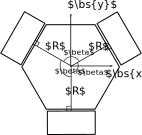
\includegraphics[width=1\linewidth]{\picPath/Screenshots/cart.png}
\end{center}
  \caption{ модель робота в программе Gazebo, использующая роликонесущие колеса для передвижения}
  \label{Figure:cartGazebo}
\end{figure}

ROS имеет две основные «стороны»: стороны операционной системы ros, как описано выше и ros-pkg, набор поддерживаемых пользователями пакетов (организованных в наборы, которые называются стек), которые реализуют различные функции робототехники: SLAM, планирование, восприятие, моделирование и др.

ROS выпускается в соответствии с условиями BSD-лицензии и c открытым исходным кодом. ROS бесплатен для использования, как в исследовательских, так и в коммерческих целях. Пакеты из ros-pkg распространяются на условиях различных открытых лицензий.
Gazebo - это трехмерный симулятор для робототехники с открытым исходным кодом. Gazebo был компонентом в Player Player с 2004 по 2011 год. Gazebo интегрировал в себя физический движок ODE, используя для рендеринга OpenGL и код поддержки для симуляции датчика и управления исполнительным механизмом. В 2011 году «Gazebo» стала независимым проектом при поддержке Willow Garage. В 2012 году Open Source Robotics Foundation (OSRF) стал руководителем проекта « Gazebo ». OSRF изменила свое название на Open Robotics в 2018 году. 


Для того, чтобы описать робота в системе Ros, необходимо задать все его параметры в специальном виде - urdf Universal Robotic Description Format).
URDF является, по сути, диалектом XML. Данный язык представляет робота как совокупность звеньев (link), сочленений (joint), сенсоров и ряда вспомогательных параметров.

Описание звена в общем виде может быть представлено следующим образом. Блок visual содержит видимую модель робота, т.е. описывает его геометрию и свойства поверхности. Геометрия может быть задана как простейшими формами (цилиндр, параллелепипед), так и сеткой, полученной в CAD-системе. Блок collision описывает ту модель, которая будет использована при выявлении столкновений с другими объектами. Чаще всего эта часть совпадает с описанием блока visible, но может и отличаться. Например, для ускорения расчётов сложный профиль поверхности может быть аппроксимирован каким-либо примитивом. В блоке inertial содержатся физические свойства звена, такие как масса или инерция.

\begin{verbatim}
<link name="link name">
  <visual>
    ... (geometry model)
  </visual>
  <collision>
    ... (collision model)
  </collision>
  <inertial>
    ... (phisical proporties)
  </inertial>
</link>
\end{verbatim}


Если робот содержит более одного звена, его элементы должны быть соединены. Для этого служат сочленения, минимальное описание которых включает в себя указание родительского звена, а также звена-потомка. Также, необходимо определить тип соединения: revolute - для вращательных, prizmatic - для призматических, continuous - для колёс, fixed - если закрепление неподвижное.


\begin{verbatim}
<joint name="joint name" type="joint type">
  <parent link="parent link name" /> 
  <child link="child link name"/>
</joint>
\end{verbatim}

Во время работы,  система ROS создает сеть, состоящую из узлов (nodes) . Пример такой сети можно видеть на рисунке \ref{Figure:rosTopic}.

\begin{figure}[H]
\begin{center}
\includegraphics[width=0.8\linewidth]{\picPath/Screenshots/rostopic.png}
\end{center}
  \caption{ граф коммуникации узлов во время тестирования}
  \label{Figure:rosTopic}
\end{figure}

 Узел- процесс, производящий вычисления. Обычно в системе много узлов для управления различными функциями. Хорошей практикой считается большое количество узлов, которые предоставляют малую функциональность, а не один большой узел, имеющий широкий функционал. узлы связываются друг с другом через сообщения. Сообщение содержит данные, которые предоставляют информацию другим узлам. ROS имеет много типов сообщений.


\newpage
\begin{center}
\bfseries Заключение
\end{center}

При выполнения преддипломной работы были рассмотрены основные подходы для решения данной проблемы.Были разработаны модель роликонесущего колеса, механическая и кинематичесая модели тележек, опирающихся на $N$ роликонесущих колес, $N>2$, изучены и обозрены методы управления роботизированными системами. Полученные сведения протестированы на виртуальной модели робота с учетом всех физических сил, воздействующих на систему. Изучен программный интерфейс систем Ros и Gazebo, разработана модель трехколесного робота, использующего для движения омни-колеса.

\newpage
%список литературы
\addcontentsline{toc}{chapter}{Список использованных источников}
\begin{thebibliography}{0}

\bibitem{Src:Siegwart}           	
Roland Siegwart
Illah R. Nourbakhsh.
Introduction to Autonomous Mobile Robots
$-$ М: The MIT Press, 2004. $-$ 321c.

\bibitem{Src:MecanumWheel}
Klaus Zimmermann, Igor Zeidis, Mohamed Abdelrahman.
Dynamics of Mechanical Systems
with Mecanum Wheels
$-$ M:  Springer International Publishing Switzerland, 2014. $-$ 11с.

\bibitem{Src:Ozhigov}
С. И. Ожегов.
Словарь русского языка
$-$ M: Мир и Образование, 2008. $-$ 1200с.


\bibitem{Src:WheelCmp}
Ksenia Shabalina, Artur Sagitov, Evgeni Magid.
Comparative Analysis of Mobile Robot Wheels
Design
$-$ M: Higher School of Information Technology and Information Systems
Kazan, Russian Federation, 2018. $-$ 5c.

\bibitem{Src:Saveliev}
И.В.Савельев.
Курс общей физики, том I.
Механика, колебания и волны, молекулярная физика.
$-$ М: Наука, 1970. $-$ 517c.

\bibitem{Src:RosBook}
Anil Mahtani, Aaron Martinez Romero.
Effective Robotics Programming with ROS - Third Edition
$-$ M: Packt, 2016. $-$ 468с.

\end{thebibliography}

\end{document}